\section{Initial Work}\label{sec:initial_work}
We have done some initial work for addressing text mining problems in business process in two use cases:

\subsection{Natural Language Generation (NLG)}

\subsubsection{Obituary Generation}
In the ongoing Interface funded project of Obituary generation at CSDM school, we are working to generate the obituary of a deceased person based on the details given about the person. We have collected the data of obituaries from one of the most famous obituary website of UK named Funeral Notices \footnote{\url{http://funeral-notices.co.uk/}}. We have selected notices only from the Scotland area and those posted after 2015. 

In the initial phase we are taking a Case-Based approach where the problem set is represented with the various features related to deceased person's life, family and funeral details. One of the commencing tasks for this approach is to develop a labelled dataset with all the features marked in the funeral notices. 
% This approach can also be termed as template filling approach.

The work is currently in progress and after the CBR implementation, we are going to take a Natural Language Generation (NLG) approach using deep learning to generate the new text based on the features given as the input to the model. 
% We will be using the transformers trained on huge datasets with millions of hyper-parameters by fine-tuning them on our custom dataset.

\subsection{Text Classification}

\subsubsection{Compliance Management}
In the recent OGIC funded AZOTH project at CSDM school, we worked on the knowledge extraction and requirement mapping on Oil and Gas regulatory documents. One of the problem statement was to identify if an extracted sentence from a document is a Compliance Requirement (CR) or not? The dataset consists of 2,600 sentences which have been determined as: 

\begin{enumerate}
    \item accept (known CR);
    \item postpone (possible CR but requires further review); and 
    \item reject (known non-CR); with respect to their CR status. 
\end{enumerate}

As a result, this is considered a classification problem of three classes. Given the arbitrary nature of the postpone class (`postpone' can be later determined as `accept' or `reject'), we modify the CR status to give two class problems. Three variants of CR status for classification are as follows:

\begin{enumerate}
    \item Accept - Reject - Postpone (3 classes): as in the original dataset as `accept', `postpone' and `reject' respectively.
    \item Not reject - Reject (2 classes): `postpone' is added to the `accept' class.
    \item Accept - Reject (2 classes): `postpone' is added to the `reject' class.
\end{enumerate}

We compared three different representation of the text to solve this problem; Linguistic features (\cref{sec:ling_ftrs}), TF-IDF vectors (\cref{sec:tfidf}) and Word2Vec Word Embeddings (\cref{sec:word_emb}). The results are shown in \cref{tab:azoth_res1}.

% \begin{table}
% 	\centering
% 	\caption{POC Verification result on 3 class problem.}\label{tab:3class_res}
% 	\begin{tabular}{|l|l|l|}
% 		\hline
% 		{\bfseries Representation} & {\bfseries Accuracy} & {\bfseries Macro F1} \\
% 		\hline
% 		{\bfseries TF-IDF} & 67.4\% & 59.3\% \\
% 		\hline
% 		{\bfseries Word2Vec} & 74.9\% & \textbf{71.5\%} \\
% 		\hline
% 		{\bfseries Linguistic Features} & \textbf{85.0\%} & 69.0\% \\
% 		\hline
% 	\end{tabular}
% \end{table}

\begin{table}
	\centering
	\caption{Compliance Requirement Verification on different class combinations.}\label{tab:azoth_res1}
	\begin{tabular}{|l|l|l|l|}
		\hline
		{\bfseries Combination} & {\bfseries Representation} & {\bfseries Accuracy} & {\bfseries Macro F1}\\
		\hline

		{\bfseries All 3 Classes} & {\bfseries TF-IDF} & 67.4\% & 59.3\% \\
		& {\bfseries Word2Vec} & 74.9\% & \textbf{71.5\%} \\
		& {\bfseries Linguistic Features} & \textbf{85.0\%} & 69.0\% \\
		\hline
		
		{\bfseries Reject vs Not-Reject} & {\bfseries TF-IDF} & 89.8\% & 80.5\%\\
		 & {\bfseries Word2Vec} & 91.5\% & 86.4\%\\
		 & {\bfseries Linguistic Features} & {\bfseries 94.0\%} & {\bfseries92.0}\%\\
		\hline
		
		{\bfseries Accept vs Reject} & {\bfseries TF-IDF} & 87.9\% & 85.5\%\\
		 & {\bfseries Word2Vec} & {\bfseries 90.6\%} & {\bfseries 88.1\%}\\
		 & {\bfseries Linguistic Features} & 89.0\% & 88.0\%\\
		\hline

	\end{tabular}
\end{table}

\subsubsection{Weighted Ensemble of Text Classifiers}\label{sec:wetc}
We have done some work in the direction of developing techniques for suitable for performing with less training data in text classification as well. Here we have used a weighted ensemble of different machine learning classifiers to classify different types of text datasets with number of training examples varying from 5k (Reuters-21578) to 5.6M (Dbpedia). The results are shown in \cref{fig:wetc_res} where we have compared our WETC algorithm with various baselines and two deep learning benchmarks BERT and ULMFiT. Newsgroup has 8k of training samples whereas Reuters has 5k and Deception has 1.2k samples only. Ag News and Dbpedia have 1.2M and 5.6M training samples respectively.

From the \cref{fig:wetc_res} we can see that our ensemble method is working better for less training data whereas deep learning algorithms are better in case of datasets with large training samples.

% \begin{table}
% 	\centering
% 	\caption{Weighted Ensemble of Text Classifiers Result}\label{tab:wetc}
% 	\begin{tabular}{|l|l|l|l|l|l|}
% 		\hline
% 		{\bfseries Algorithms} & {\bfseries Reuters} & {\bfseries Newsgroup} & {\bfseries Decption} & {\bfseries Ag News} & {\bfseries Dbpedia} \\
% 		\hline
% 		{\bfseries WETC} & 67.4\% & 59.3\% & & & \\
% 		\hline
% 		{\bfseries Random Forest} & 74.9\% & \textbf{71.5\%} & & & \\
% 		\hline
% 		{\bfseries Xg Boost} & 74.9\% & \textbf{71.5\%} & & & \\
% 		\hline
% 		{\bfseries Naive Bayes} & 74.9\% & \textbf{71.5\%}  & & & \\
% 		\hline
% 		{\bfseries Logistic Regression} & 74.9\% & \textbf{71.5\%}  & & & \\
% 		\hline
% 		{\bfseries SVM} & 74.9\% & \textbf{71.5\%}  & & & \\
%         \hline
% 		{\bfseries BERT} & 74.9\% & \textbf{71.5\%}  & & & \\
% 		\hline
% 		{\bfseries ULMFiT} & \textbf{85.0\%} & 69.0\%  & & & \\
% 		\hline
% 	\end{tabular}
% \end{table}

\begin{figure}
    \centering
    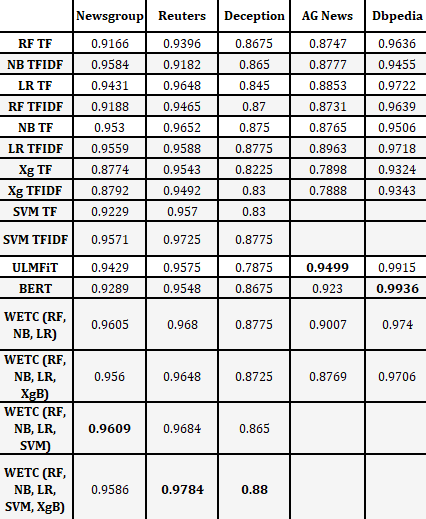
\includegraphics[width=0.75\textwidth]{images/wetc.png}
    \caption{Weighted Ensemble of Text Classifiers Result}
    \label{fig:wetc_res}
\end{figure}


% The results from \cref{tab:azoth_res1} suggest that the hand crafted deep learning methods are equally better as of the linguistic features. The graph from the \cref{fig:azoth_res1} and \cref{fig:azoth_res2} suggest that with the increase in data, the performance of the model changes as well. We can see the class imbalance problem from the \cref{fig:azoth_res1} and \cref{fig:azoth_res2} when in the last step, where whole data is being used for training we can see a drop in macro f1 score where as a rise in the accuracy. This is due to the fact that the dataset is heavily imbalanced (1500 examples for accept, 600 for postpone and 400 for reject).

% \begin{figure}
%     \centering
%     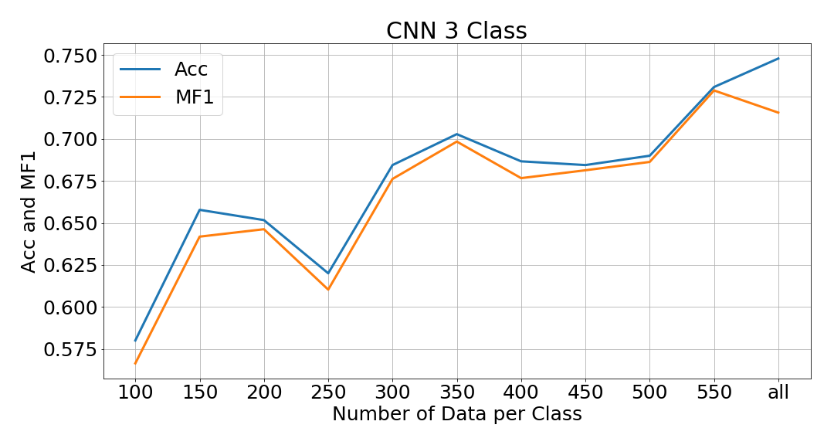
\includegraphics[width=\textwidth]{images/cnn3class.png}
%     \caption{CNN change in performance w.r.t change in data per class in 3 class problem}
%     \label{fig:azoth_res1}
% \end{figure}

% \begin{figure}
%     \centering
%     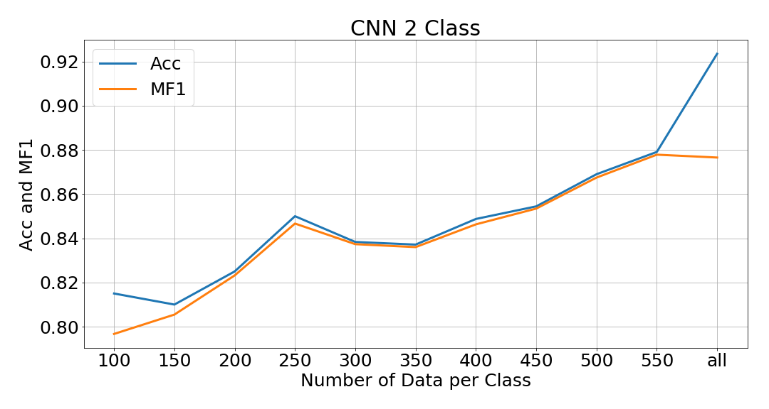
\includegraphics[width=\textwidth]{images/cnn2.png}
%     \caption{CNN change in performance w.r.t change in data per class in accept vs reject}
%     \label{fig:azoth_res2}
% \end{figure}

